\newcommand{\crel}{%
	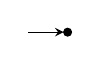
\begin{tikzpicture}[baseline={([yshift=-.8ex]current bounding box.center)}]
		\draw [->, >=stealth] (0,0) -- (0.45,0); 
		\draw [fill] (0.5,0) circle (0.05);
	\end{tikzpicture}
}

\newcommand{\rrel}{%
	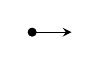
\begin{tikzpicture}[baseline={([yshift=-.8ex]current bounding box.center)}]
		\draw [fill] (0,0) circle (0.05);
		\draw [->, >=stealth] (0.05,0) -- (0.5,0);
	\end{tikzpicture}
}

\newcommand{\mrel}{%
	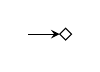
\begin{tikzpicture}[baseline={([yshift=-.8ex]current bounding box.center)}]
		\draw [->, >=stealth] (0,0) -- (0.4,0);
		\draw (0.4,0) -- (0.475,0.075) -- (0.55,0) -- (0.475,-0.075) -- cycle;
	\end{tikzpicture}
}

\newcommand{\irel}{%
	\begin{tikzpicture}[baseline={([yshift=-.8ex]current bounding box.center)}]
		\draw [->, >=stealth] (0,0) -- (0.4,0);
		\draw (0.41,0) -- (0.55,0);
		\draw (0.48,-0.07) -- (0.48, 0.07); 
	\end{tikzpicture}
}

\newcommand{\erel}{%
	\begin{tikzpicture}[baseline={([yshift=-.8ex]current bounding box.center)}]
		\draw [->, >=stealth] (0,0) -- (0.4,0);
		\draw (0.41,0) -- (0.55,0);
		\draw (0.48, 0.05) circle (0.02);
		\draw (0.48, -0.05) circle (0.02); 
	\end{tikzpicture}
}

\newcommand{\ev}[2][001]{% {Executed Pending Included} Name
\StrMid{#1}{1}{1}[\posone]%
\StrMid{#1}{2}{2}[\postwo]%
\StrMid{#1}{3}{3}[\posthree]%
\begin{tikzpicture}[baseline={([yshift=-.8ex]current bounding box.center)}]

% Executed tick
\ifthenelse{\equal {\posone} {1}}
{\draw (0.275, 0.1) -- (0.305, 0.07) -- (0.365, 0.12);}
{}

% Pending exclamation
\ifthenelse{\equal {\postwo} {1}}
{\draw (0.31, 0.26) -- (0.31, 0.18);
\draw[fill] (0.31, 0.16) circle [radius=0.005];}
{}

% Box
\ifthenelse{\equal {\posthree} {1}}
{\draw (0, 0) -- (0.4, 0) -- (0.4, 0.3) -- (0, 0.3) -- (0, 0);}
{
\draw (0, 0.2550) -- (0, 0.1950);
\draw (0, 0.1800) -- (0, 0.1200);
\draw (0, 0.1050) -- (0, 0.0450);
\draw (0, 0.27) -- (0, 0.3) -- (0.03, 0.3); % Top left
\draw (0.0450, 0.3) -- (0.11125, 0.3);
\draw (0.12625, 0.3) -- (0.1925, 0.3);
\draw (0.2075, 0.3) -- (0.27375, 0.3);
\draw (0.28875, 0.3) -- (0.355, 0.3);
\draw (0.37, 0.3) -- (0.4, 0.3) -- (0.4, 0.27); % Top right		
\draw (0.4, 0.2550) -- (0.4, 0.1950);
\draw (0.4, 0.1800) -- (0.4, 0.1200);
\draw (0.4, 0.1050) -- (0.4, 0.0450);
\draw (0.37, 0) -- (0.4, 0) -- (0.4, 0.03); % Bottom right
\draw (0.0450, 0) -- (0.11125, 0);
\draw (0.12625, 0) -- (0.1925, 0);
\draw (0.2075, 0) -- (0.27375, 0);
\draw (0.28875, 0) -- (0.355, 0);
\draw (0, 0.03) -- (0, 0) -- (0.03, 0); % Bottom left
}

% Name
\node [name] at (0.15, 0.15) {\texttt{#2}};
\end{tikzpicture}%
}
